\chapter{LAB 04: Process Termination and WaitPID}

\section{Introduction: The Interconnected Process Lifecycle}
In OS161, a process terminates by invoking the \texttt{exit()} standard library function, which triggers the \texttt{SYS\_exit} system call. Conversely, \textbf{\texttt{waitpid()} is the specific function in charge of waiting for the termination of a spawned child process}. A parent process calls \texttt{waitpid()} to pause its own execution until its child finishes, and then reads the child's exit status.

But \textit{why} must a parent wait for its child?
\begin{itemize}
    \item \textbf{Synchronization:} A parent often cannot safely proceed until the child completes its task. For instance, a shell program must wait for a user's command to finish executing before printing the next prompt, otherwise the terminal output would become chaotically interleaved.
    \item \textbf{Control Flow:} The parent needs to read the child's exit status to know if the execution succeeded or failed, which dictates the parent's next logical step.
\end{itemize}

This requirement creates a domino effect of interconnected mechanisms:
\begin{enumerate}
    \item We need the child's exit status to survive after the child dies. This requires the \textbf{Zombie State}.
    \item We need the parent to be able to locate this Zombie from user-space. This requires assigning a unique integer identifier, the \textbf{PID}.
    \item The kernel must rapidly map this PID to the Zombie's memory location. This necessitates a global \textbf{Process Table}.
    \item To avoid confusing parents with stale data, we must assign PIDs safely. This demands a \textbf{Circular Buffer} algorithm.
\end{enumerate}
This laboratory explores the intricate dance between \texttt{sys\_exit} and \texttt{sys\_waitpid}, demonstrating how these structures depend on one another.

\begin{figure}[htbp]
    \centering
    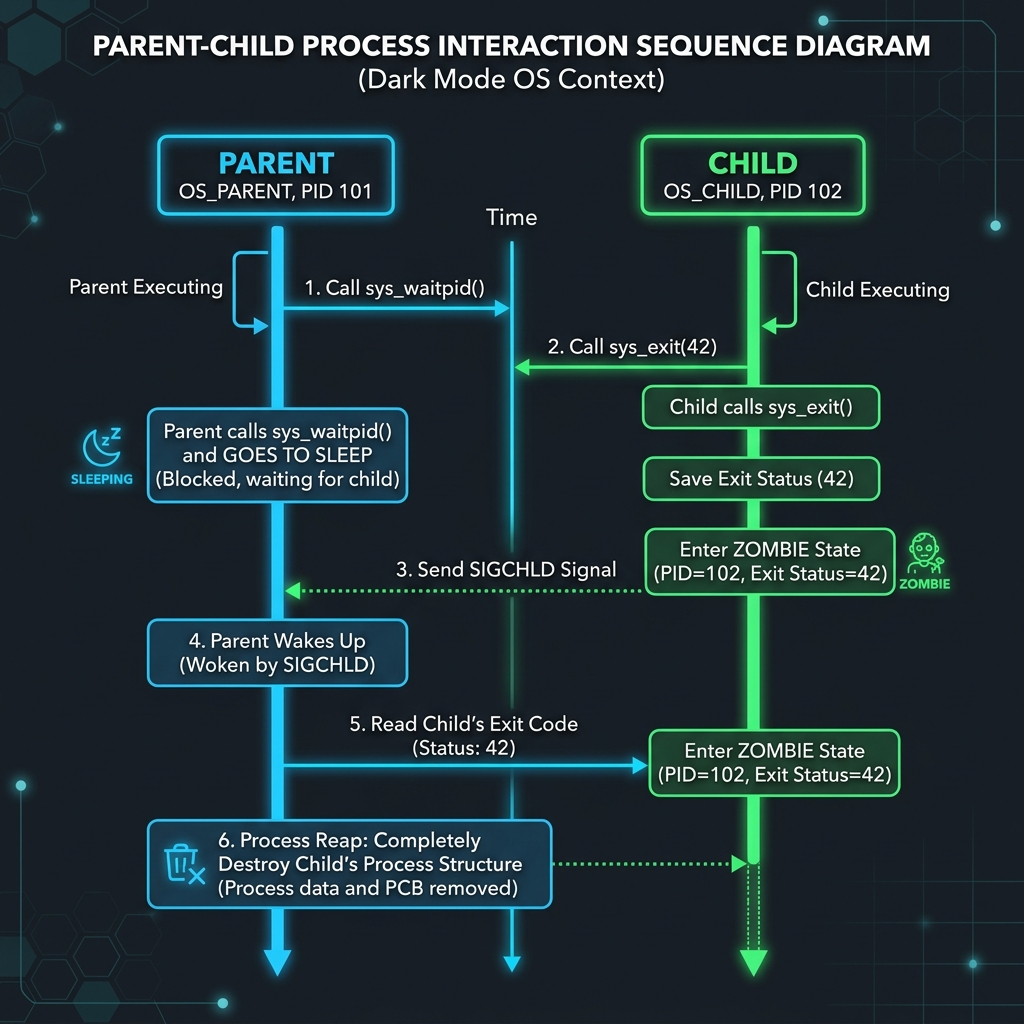
\includegraphics[width=\textwidth]{images/exit_waitpid_dance.png}
    \caption{The synchronization sequence between a parent calling \texttt{waitpid} and a child calling \texttt{exit}.}
\end{figure}

\section{The Process Table and PID Assignment}
To implement \texttt{waitpid(pid)}, the kernel must convert an integer PID into a \texttt{struct proc *} pointer in $O(1)$ time. 

\subsection{High-Level Structure: The Process Table}
We expect the Process Table to be a global array protected by a spinlock. The PID assigned to a process will literally be its index in this array.
\begin{lstlisting}[language=C]
// Expected High-Level Structure
struct _processTable {
  struct proc *proc[MAX_PROC + 1]; // Array of process pointers
  int last_i;                      // Tracks the last assigned PID
  struct spinlock lk;              // Mutual exclusion lock
} processTable;

// Expected Conversion Function
struct proc *proc_search_pid(pid_t pid) {
    // 1. Check if PID is within bounds
    // 2. Acquire processTable.lk
    // 3. Extract processTable.proc[pid]
    // 4. Release processTable.lk
    // 5. Return the extracted pointer
}
\end{lstlisting}

\subsection{Circular Buffer for PID Assignment}
A naive approach to finding a free PID is to always scan the Process Table from index 1 to \texttt{MAX\_PROC} and return the very first empty slot. However, this leads to \textbf{rapid PID reuse}. If Process 1 dies and is reaped, the very next process spawned will immediately become Process 1. 

\textbf{Why is rapid PID reuse dangerous?}\\
A common misconception is that when a child terminates, the parent is instantly and actively notified. This is not how Unix works. When a child terminates, it becomes a \textbf{Zombie}; its exit status sits passively in the process table until the parent explicitly decides to call \texttt{waitpid}. 

Even after the parent reaps the child (finally freeing the PID), rapid reuse is dangerous due to \textbf{stale references} and \textbf{asynchronous signals}:
\begin{itemize}
    \item \textbf{Stale References (The Bug):} Imagine a parent process tracks its child's PID (e.g., PID 5). The child dies, and the parent reaps it. PID 5 is now free. Immediately, a completely different user program spawns a new process, which is assigned the newly freed PID 5. If the original parent has a logic bug and mistakenly calls \texttt{kill(5)} or \texttt{waitpid(5)} \textit{again} (thinking it is still targeting its child), it will accidentally kill or block on an innocent, unrelated process! 
\end{itemize}

To visualize what we expect from the Circular Buffer algorithm to mitigate this:
\begin{lstlisting}[language=C]
// Expected Circular Assignment Logic
pid_t assign_pid(struct proc *new_proc) {
    // 1. Start searching from (last_i + 1)
    // 2. Loop until we find an index where processTable.proc[i] == NULL
    // 3. If we hit MAX_PROC, wrap around back to 1
    // 4. Save new_proc at that index, update last_i, and return the PID
}
\end{lstlisting}
This guarantees that a PID is only reused after \texttt{MAX\_PROC} other processes have been spawned, drastically reducing the chance of stale reference bugs.

\section{The Exit System Call and the Zombie State}
When a user program calls \texttt{sys\_exit(int status)}, the kernel must perform cleanup. 

\subsection{The Zombie State}
The Zombie state is the critical mechanism that allows a parent process to reliably capture the exit status of a terminated child. To understand why it is so important, consider the catastrophic bugs that would occur if a dying process directly called \texttt{proc\_destroy(curproc)} instead of becoming a zombie:

\begin{itemize}
    \item \textbf{Endless Waiting / Lost Status:} If the child completely destroyed itself, its exit status would be instantly erased. Furthermore, if the parent later calls \texttt{waitpid()} and attempts to sleep on the child's Condition Variable, but that CV was just wiped from memory by the child's suicide, the parent will either crash or block endlessly waiting for a signal from a thread that no longer exists!
    \item \textbf{The Suicide Paradox:} A dying process executes \texttt{sys\_exit} using the kernel stack attached to its own thread. If it calls \texttt{proc\_destroy(curproc)}, it deallocates its own memory structure while still running code on it, causing an immediate kernel panic (a memory fault).
\end{itemize}

Instead, the process enters the \textbf{Zombie State}. It is dead, but its \texttt{struct proc} skeleton remains safely preserved in the Process Table, holding the exit status. It is the strict responsibility of the \textit{parent} process (via \texttt{waitpid}) to finally read the status and completely obliterate the child.

\begin{figure}[h]
    \centering
    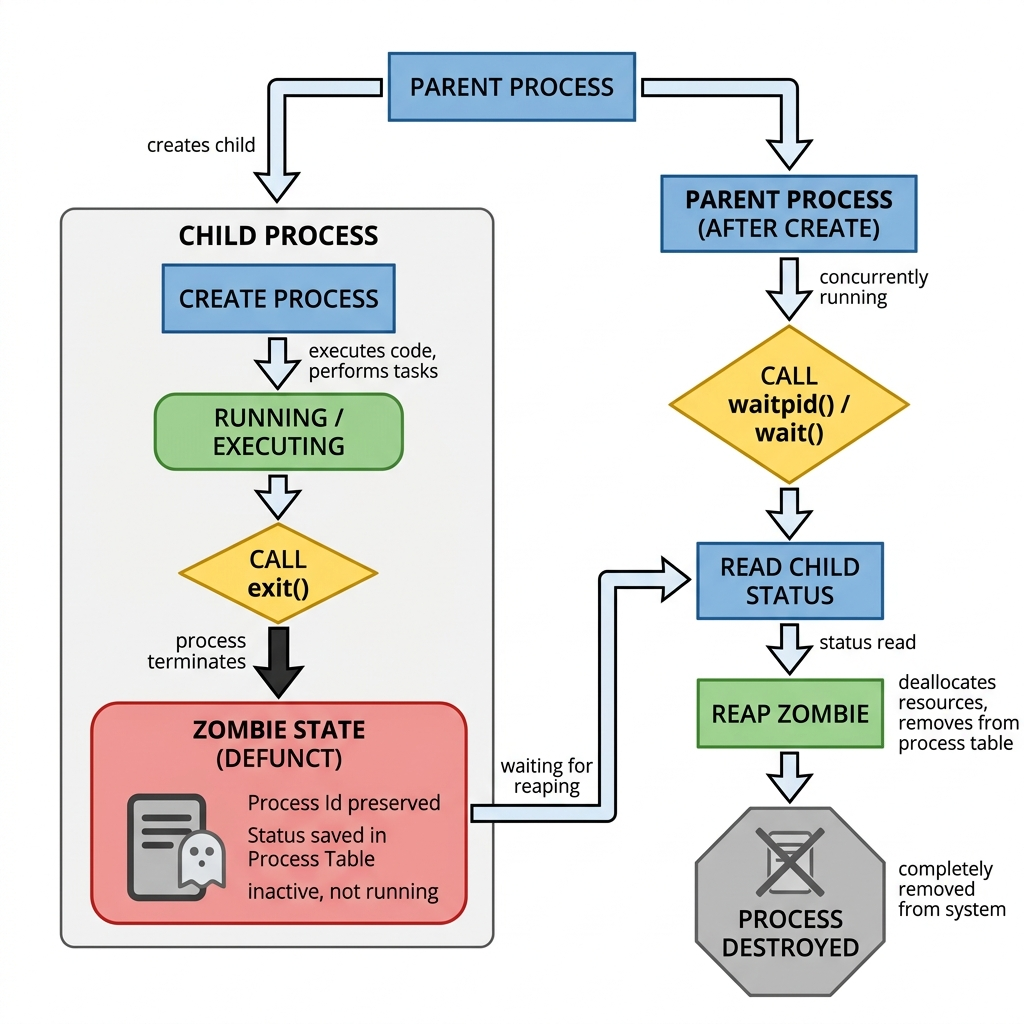
\includegraphics[width=0.8\textwidth]{images/zombie_process_lifecycle.png}
    \caption{Process lifecycle showing the transition into the Zombie state and subsequent reaping by the parent.}
    \label{fig:zombie_lifecycle}
\end{figure}

\begin{lstlisting}[language=C]
// Expected sys_exit Structure
void sys__exit(int status) {
    // 1. Save the status inside curproc->p_status
    // 2. Detach the thread from the process
    // 3. Signal the parent process that we are dying
    // 4. Call thread_exit() to kill the thread. 
    //    (The proc structure survives as a Zombie!)
}
\end{lstlisting}

\subsection{The Thread Termination Rule and the Race Condition}
A critical rule in OS161 is that \textbf{a process cannot be destroyed until all the threads it spawned have ended} (\texttt{p\_numthreads == 0}). 

This creates a subtle but fatal race condition inside \texttt{sys\_exit}. If \texttt{sys\_exit} signals the parent \textit{before} explicitly detaching its thread, the parent might wake up and destroy the process while the child thread is still executing its final instructions.

\textbf{Visualizing the Bug (The Race Condition Sequence):}

\begin{figure}[h]
    \centering
    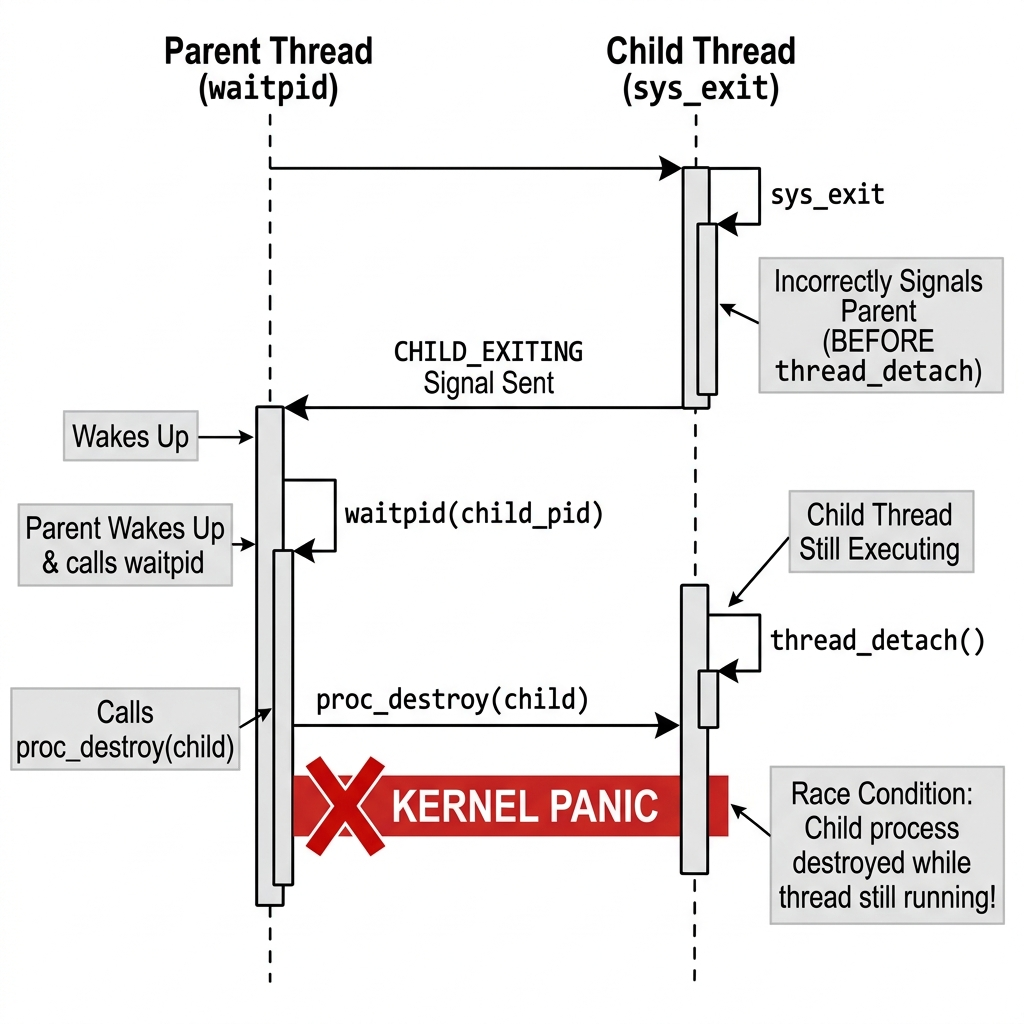
\includegraphics[width=0.8\textwidth]{images/sys_exit_race_condition.png}
    \caption{Sequence diagram illustrating the race condition in sys\_exit if the parent is signaled before thread detachment.}
    \label{fig:race_condition}
\end{figure}

\begin{verbatim}
      CHILD THREAD (sys_exit)                  PARENT THREAD (waitpid)
------------------------------------     ------------------------------------
1. curproc->p_status = status;           1. cv_wait(child->p_cv); (Sleeping)
2. cv_signal(curproc->p_cv);  =========> 2. WAKES UP!
3. (Context Switch / Preempted)          3. proc_destroy(child_proc);
                                         4. KASSERT(child->p_numthreads == 0);
                                            ^^^^^^^^^^^^^^^^^^^^^^^^^^^^^^^^
                                            KERNEL PANIC! Assertion fails 
                                            because Child Thread hasn't 
                                            called proc_remthread yet!
\end{verbatim}

To fix this, \texttt{sys\_exit} must \textbf{manually and explicitly call \texttt{proc\_remthread(curthread)}} \textit{before} firing the signal. This detaches the thread, decrementing \texttt{p\_numthreads} to 0, ensuring the parent's assertion will safely pass even if the child thread is still technically finishing its jump to the graveyard.

\section{The Wait System Call: \texttt{sys\_waitpid} vs \texttt{proc\_wait}}
For pedagogical clarity, the waiting logic is split into two distinct layers: User and Kernel.

\subsection{User Layer: \texttt{sys\_waitpid}}
This is the system call handler. It receives a raw integer \texttt{pid} from user space. 
\begin{lstlisting}[language=C]
// Expected sys_waitpid Structure
int sys_waitpid(pid_t pid, userptr_t statusp) {
    // 1. Use proc_search_pid(pid) to get the struct proc pointer
    // 2. Call the internal kernel function: proc_wait(target_proc)
    // 3. Safely copyout() the returned status to the userptr_t
}
\end{lstlisting}

\subsection{Kernel Layer: \texttt{proc\_wait}}
This function operates purely on kernel pointers and contains the actual synchronization logic.

\textbf{Condition Variables vs Semaphores for Synchronization}\\
A parent process waiting for its child \textbf{must be evicted} from the CPU (put to sleep); otherwise, it will endlessly consume CPU cycles in a busy-waiting loop, destroying system performance. There are two primary synchronization primitives that can achieve this:
\begin{itemize}
    \item \textbf{Semaphores (\texttt{USE\_SEMAPHORE\_FOR\_WAITPID}):} A semaphore initialized to 0 is an elegant solution. The parent simply calls \texttt{P(child->p\_sem)} to sleep, and the exiting child calls \texttt{V(child->p\_sem)} to wake the parent.
    \item \textbf{Condition Variables:} If using a CV, a thread cannot simply go to sleep while holding a standard lock (mutex), because the child process will need to acquire that exact same lock in order to send the wake-up signal. If the parent sleeps while holding the lock, the child will deadlock trying to acquire it. Therefore, the \texttt{cv\_wait} function is strictly required because it atomically puts the parent to sleep \textit{and} releases the lock, allowing the child to safely acquire it, trigger \texttt{cv\_signal}, and release it.
\end{itemize}

\begin{lstlisting}[language=C]
// Expected proc_wait Structure
int proc_wait(struct proc *child_proc) {
    // 1. Acquire the child's lock
    // 2. Sleep on the child's condition variable (cv_wait)
    // 3. Wake up, read child_proc->p_status
    // 4. Call proc_destroy(child_proc) to REAP THE ZOMBIE!
    // 5. Return the status
}
\end{lstlisting}

\begin{tcolorbox}[colback=blue!5!white,colframe=blue!75!black,title=Exam Insight: Process vs Thread Creation (e.g. Q4 2023-06-20)]
\textbf{thread\_switch vs thread\_fork:} When creating a new executing entity, it is vital to distinguish between these functions. \texttt{thread\_switch} does \textbf{not} create anything; it is simply the low-level assembly routine that performs the context switch (saving and restoring CPU registers). \texttt{thread\_fork}, instead, allocates and creates the actual kernel thread structure. However, to create a full \textit{process}, both a process structure (via \texttt{proc\_create}) and a thread (via \texttt{thread\_fork}) must be created and linked together.

\textbf{Thread Ownership on Fork:} When \texttt{thread\_fork(const char *name, struct proc *proc, ...)} is called, the newly minted thread belongs to the process passed as the \texttt{proc} parameter. It \textbf{does not} automatically belong to the calling process! For instance, during a \texttt{sys\_fork}, the parent process executes the \texttt{thread\_fork} call, but passes a pointer to the newly created \textit{child} \texttt{proc} structure. Thus, the new thread correctly belongs to the child process, not the parent that physically invoked the function.
\end{tcolorbox}

\section{Applying Wait Logic to the Kernel Menu}
In the baseline OS161 distribution, if you execute a user program from the kernel menu (e.g., \texttt{p testbin/add}), the kernel spawns a new thread via \texttt{common\_prog} and immediately returns to the menu prompt while the program is still running, cluttering the console.

We expect to patch \texttt{common\_prog} so it waits for the program to finish. But why does \texttt{common\_prog} directly call \texttt{proc\_wait} instead of the official \texttt{sys\_waitpid}? 

Because \texttt{sys\_waitpid} is strictly a \textbf{user-space wrapper}. Its entire purpose is to safely transition a user program into the kernel: it validates user privileges, translates an integer PID into a kernel pointer using the Process Table, and securely uses \texttt{copyout} to send the integer status back to user memory. 

Since \texttt{common\_prog} is the OS kernel menu, it is already executing with full kernel privileges. It doesn't need to perform user-space security checks, it doesn't need \texttt{copyout}, and it doesn't even need to deal with PIDs because it directly possesses the raw \texttt{struct proc *} pointer returned by \texttt{proc\_create\_runprogram}. Therefore, it completely bypasses the \texttt{sys\_waitpid} wrapper and directly invokes the internal kernel engine: \texttt{proc\_wait(child\_proc)}.

\begin{lstlisting}[language=C]
// Expected common_prog Patch
int common_prog(int argc, char **argv) {
    struct proc *proc = proc_create_runprogram(argv[0]);
    // ... thread_fork occurs here ...
    
    // NEW: Synchronize the menu by waiting for the child to die!
    proc_wait(proc); 
    return 0;
}
\end{lstlisting}

\newpage
\section{Laboratory 04: Step-by-Step Guide}


\subsection{The Goal and the Current Problem}
Currently, OS161 cannot execute user programs cleanly. If you run a program, the kernel does not wait for it to finish. If the program attempts to call \texttt{exit()}, the system crashes because the termination logic is incomplete. 
Our goal is to implement the Process Table, PID management, and the synchronization dance between \texttt{sys\_exit} and \texttt{sys\_waitpid} to allow processes to terminate cleanly as Zombies, and for parents to safely wait and read their exit status.

\subsection{Step 1: Upgrading the Process Structure}
Open \texttt{kern/include/proc.h}. By default, the \texttt{struct proc} only contains fields for memory (\texttt{p\_addrspace}), threads (\texttt{p\_numthreads}), and the filesystem (\texttt{p\_cwd}). There is literally nowhere to store an exit status or a PID. We cannot store the exit status inside the thread structure because the thread is destroyed long before the parent calls \texttt{waitpid}. Therefore, we must explicitly add \texttt{p\_status} and \texttt{p\_pid}. 

Furthermore, we need a way for the parent to safely sleep while waiting for the child to die. We cannot use the existing \texttt{struct spinlock p\_lock} for this, because threads are strictly forbidden from sleeping while holding a spinlock. Thus, we must introduce a high-level \texttt{struct lock *} and a \texttt{struct cv *} dedicated solely to this wake-up mechanism.
\begin{lstlisting}[language=C]
struct proc {
    char *p_name;
    struct spinlock p_lock;
    unsigned p_numthreads;
    struct addrspace *p_addrspace;
    struct vnode *p_cwd;

    /* Added for Lab 04: Waitpid & Exit Support */
    int p_status;        /* Exit status returned by sys_exit */
    pid_t p_pid;         /* Process Identifier */
    
    struct cv *p_cv;     /* CV to signal the waiting parent */
    struct lock *p_lock; /* Lock protecting the CV */
};
\end{lstlisting}

\subsection{Step 2: Defining the Process Table}
Open \texttt{kern/proc/proc.c}. While we could theoretically link all processes in a linked list, \texttt{sys\_waitpid} needs to find a process instantly based on an integer PID. An array of pointers allows $O(1)$ lookups, where the index is the PID itself. We also introduce a dedicated spinlock (\texttt{processTable.lk}) because multiple CPUs might attempt to spawn or destroy processes at the exact same nanosecond; without mutual exclusion, the array would become corrupted.
\begin{lstlisting}[language=C]
#define MAX_PROC 100
static struct _processTable {
  int active;
  struct proc *proc[MAX_PROC + 1]; /* [0] not used. pids are >= 1 */
  int last_i;                      /* index of last allocated pid */
  struct spinlock lk;              /* Lock for this table */
} processTable;
\end{lstlisting}
We must initialize this table during kernel boot. Add the following to \texttt{proc\_bootstrap()}:
\begin{lstlisting}[language=C]
void proc_bootstrap(void) {
    kproc = proc_create("[kernel]");
    if (kproc == NULL) panic("proc_create for kproc failed\n");
    
    spinlock_init(&processTable.lk);
    processTable.active = 1;
}
\end{lstlisting}

\subsection{Step 3: Circular PID Assignment}
When \texttt{proc\_create} is called, we must search the Process Table for a free slot. To implement the circular buffer logic we discussed in the theory section (which prevents the stale reference bugs caused by rapid PID reuse), we add this helper function:
\begin{lstlisting}[language=C]
static void proc_init_waitpid(struct proc *proc, const char *name) {
  int i;
  spinlock_acquire(&processTable.lk);
  i = processTable.last_i + 1;
  proc->p_pid = 0;
  
  if (i > MAX_PROC) i = 1;
  while (i != processTable.last_i) {
    if (processTable.proc[i] == NULL) {
      processTable.proc[i] = proc;
      processTable.last_i = i;
      proc->p_pid = i;
      break;
    }
    i++;
    if (i > MAX_PROC) i = 1;
  }
  spinlock_release(&processTable.lk);
  
  if (proc->p_pid == 0) panic("too many processes. proc table is full\n");
  
  proc->p_status = 0;
  proc->p_cv = cv_create(name);
  proc->p_lock = lock_create(name);
}
\end{lstlisting}
Ensure this function is called at the end of \texttt{proc\_create()}.

\subsection{Step 4: Implementing \texttt{sys\_exit}}
Open \texttt{kern/syscall/proc\_syscalls.c}. When a process exits, it must perform four critical steps motivated by the Zombie architecture:
1. It must mask the status with \texttt{status \& 0xff}. (OS161, like POSIX, only uses the lower 8 bits for the actual exit code).
2. It must detach its thread \textbf{before} signaling the parent, otherwise it triggers the fatal race condition panic we visualized earlier.
3. It must wake the parent using \texttt{cv\_signal}.
4. It must call \texttt{thread\_exit()} to kill the thread, leaving the \texttt{proc} intact as a Zombie.
\begin{lstlisting}[language=C]
void sys__exit(int status) {
  struct proc *p = curproc;
  
  /* Save just the lower 8 bits returned */
  p->p_status = status & 0xff; 
  
  /* EXTREMELY IMPORTANT: Detach thread before signaling parent! */
  proc_remthread(curthread);
  
  /* Wake up the parent waiting in waitpid */
  lock_acquire(p->p_lock);
  cv_signal(p->p_cv);
  lock_release(p->p_lock);

  /* The thread dies, but the proc structure remains as a Zombie */
  thread_exit();
  panic("thread_exit returned (should not happen)\n");
}
\end{lstlisting}

\subsection{Step 5: Implementing \texttt{proc\_wait}}

\begin{tcolorbox}[colback=red!5!white, colframe=red!75!black, title=\textbf{! EXAM FOCUS: IMPLEMENTATION REQUIRED}]
\textbf{Function:} \texttt{proc\_wait(struct proc *proc)} \\
\textbf{Exam Task:} \textit{Bug Detection} \\
Exams present a buggy version of \texttt{proc\_wait} containing critical synchronization errors. You must be able to spot: 1) calling \texttt{cv\_wait} \textit{before} \texttt{lock\_acquire}, 2) returning an error status without releasing the lock (deadlock), and 3) wrongly destroying the parent \texttt{curproc} instead of the child \texttt{proc}.
\end{tcolorbox}

The parent process waits for the child by sleeping on its CV. Once awakened, the parent must read the exit status \textbf{before} calling \texttt{proc\_destroy}. This ordering is strictly motivated by memory safety: if the parent called \texttt{proc\_destroy} first, the Zombie would be obliterated, and reading \texttt{p\_status} would cause a use-after-free memory fault! Back in \texttt{proc.c}:
\begin{lstlisting}[language=C]
int proc_wait(struct proc *proc) {
    int return_status;
    KASSERT(proc != NULL);
    KASSERT(proc != curproc);

    lock_acquire(proc->p_lock);
    cv_wait(proc->p_cv, proc->p_lock);
    lock_release(proc->p_lock);

    return_status = proc->p_status;
    proc_destroy(proc);
    return return_status;
}
\end{lstlisting}

\subsection{Step 6: Table Lookup and Cleanup Functions}

\begin{tcolorbox}[colback=red!5!white, colframe=red!75!black, title=\textbf{! EXAM FOCUS: IMPLEMENTATION REQUIRED}]
\textbf{Function:} \texttt{proc\_to\_pid \& proc\_from\_pid} \\
\textbf{Exam Task:} \textit{Implement from Scratch} \\
You must know how to build the mapping between a \texttt{pid\_t} and a \texttt{struct proc *}. The exam explicitly asks you to realize these conversion functions and explain the global data structure (the process table/array) and the necessary locking synchronization required to make them thread-safe.
\end{tcolorbox}

To complete the architecture, we must implement two critical helper functions in \texttt{proc.c}. 

First, \texttt{proc\_search\_pid} is used by \texttt{sys\_waitpid} to safely extract a process pointer from the table:
\begin{lstlisting}[language=C]
struct proc *proc_search_pid(pid_t pid) {
  struct proc *p;
  KASSERT(pid >= 0 && pid < MAX_PROC);
  spinlock_acquire(&processTable.lk);
  p = processTable.proc[pid];
  spinlock_release(&processTable.lk);
  return p;
}
\end{lstlisting}

Second, when \texttt{proc\_destroy} finally obliterates the Zombie, it must free the PID slot so it can be reused later. It must also destroy the synchronization primitives we added. We isolate this in \texttt{proc\_end\_waitpid}:
\begin{lstlisting}[language=C]
static void proc_end_waitpid(struct proc *proc) {
  int i;
  spinlock_acquire(&processTable.lk);
  i = proc->p_pid;
  KASSERT(i > 0 && i <= MAX_PROC);
  processTable.proc[i] = NULL;
  spinlock_release(&processTable.lk);

  cv_destroy(proc->p_cv);
  lock_destroy(proc->p_lock);
}
\end{lstlisting}
\textbf{Important:} You must explicitly add a call to \texttt{proc\_end\_waitpid(proc);} at the very end of the \texttt{proc\_destroy()} function!

\subsection{Step 7: Enabling the WAITPID Option}
If you wrap your implementation inside the \texttt{\#if OPT\_WAITPID} macro, the compiler will completely ignore your code unless you explicitly configure the kernel to activate it.

To do this, you must modify two files:
\begin{enumerate}
    \item Open \texttt{kern/conf/conf.kern}. This tells the configuration system that the option exists. Find the other \texttt{defoption} lines and add:
    \begin{verbatim}
defoption waitpid
    \end{verbatim}
    
    \item Open your specific kernel configuration file, e.g., \texttt{kern/conf/DUMBVM}. This explicitly turns the option on for the build. Add:
    \begin{verbatim}
options waitpid
    \end{verbatim}
\end{enumerate}

When you subsequently run \texttt{./config DUMBVM}, the build system will automatically generate the header \texttt{opt-waitpid.h} containing \texttt{\#define OPT\_WAITPID 1}, effectively activating all your new code.

\subsection{Step 8: Testing the Execution}
Compile your kernel and run a simple user program like \texttt{testbin/add}:
\begin{verbatim}
$ sys161 kernel
OS/161 kernel [? for menu]: p testbin/add
\end{verbatim}
\textbf{Expected Results:} The program will execute, print the result of the addition, and then cleanly return to the OS/161 menu. Behind the scenes, the child executed \texttt{sys\_exit}, became a Zombie, and the parent (the kernel menu thread) executed \texttt{proc\_wait}, reaped the Zombie, and resumed operation without panicking.

\newpage
\section{Global Architecture: The Process Termination Call Graph}
To provide absolute clarity on the overall "dance" between process termination and synchronization, the following call graph summarizes the entire architecture.

\begin{figure}[htbp]
    \centering
    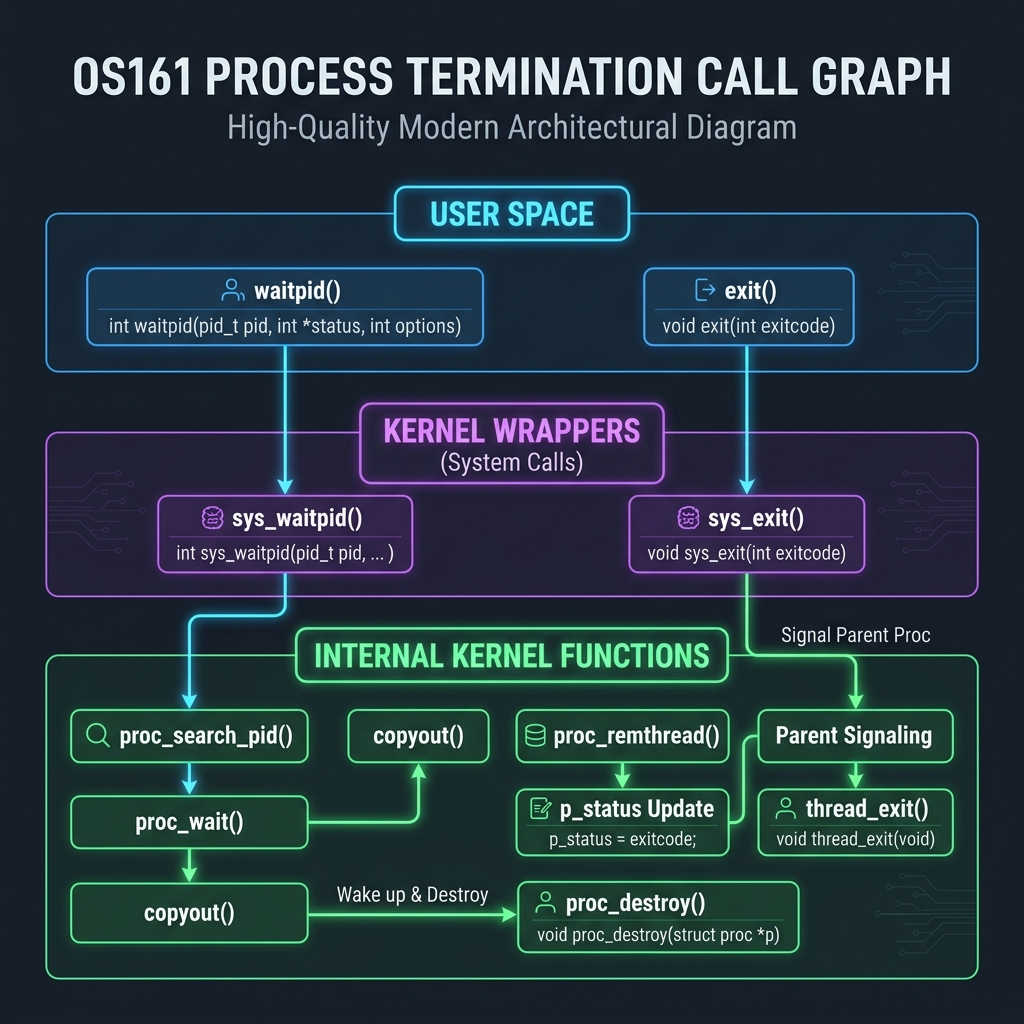
\includegraphics[width=\textwidth]{images/waitpid_exit_architecture.png}
    \caption{The architectural call graph for Process Termination and WaitPID in OS161.}
\end{figure}

The architecture is divided into three distinct layers:
\begin{enumerate}
    \item \textbf{User Space:} The user applications call the standard C library functions \texttt{waitpid()} and \texttt{exit()}. These trigger hardware traps to transition securely into the kernel.
    \item \textbf{Kernel Wrappers (\texttt{sys\_waitpid} \& \texttt{sys\_exit}):} These act as the boundary layer. They validate user pointers, translate integer PIDs into actual kernel \texttt{struct proc *} pointers using \texttt{proc\_search\_pid()}, and manage the safe transfer of data between user and kernel space (via \texttt{copyout}).
    \item \textbf{Internal Kernel Functions:} This is where the core logic executes. 
    \begin{itemize}
        \item \texttt{proc\_wait()} executes the blocking synchronization (via Semaphore or Condition Variable), pausing the parent.
        \item \texttt{sys\_exit} performs the teardown: it detaches the thread (\texttt{proc\_remthread}), updates the zombie status (\texttt{p\_status = exitcode}), signals the parent to wake up, and finally calls \texttt{thread\_exit()} to kill the executing thread.
        \item Finally, the awakened parent finishes \texttt{proc\_wait()}, returns the exit status via \texttt{copyout()}, and completely obliterates the child's data structures by calling \texttt{proc\_destroy()}.
    \end{itemize}
\end{enumerate}

\newpage

\section{The Open File Table (Preview)}

\begin{tcolorbox}[colback=red!5!white, colframe=red!75!black, title=\textbf{! EXAM FOCUS: IMPLEMENTATION REQUIRED}]
\textbf{Function:} \texttt{struct openfile} \\
\textbf{Exam Task:} \textit{Analysis \& Process Interaction} \\
Although file descriptors are covered extensively later, OS161 exams specifically ask about the interaction between the 	extbf{global} system-wide \texttt{systemFileTable} and the 	extbf{process-local} \texttt{fileTable} array inside \texttt{struct proc}. You must understand what happens when two processes have pointers to the exact same global \texttt{struct openfile} (e.g., they share the file offset during an \texttt{lseek}).
\end{tcolorbox}

\section*{Past Exam Questions}

\subsection*{Group 1: The Exit System Call and Zombies}

\textbf{[Exams 2021-07-05, 2022-09-08, 2022-10-26, 2024-07-11]}
\textit{Perché il processo che termina (con \texttt{sys\_exit}) non può chiamare direttamente la \texttt{proc\_destroy(curproc)}, dopo aver segnalato la fine del processo stesso e prima della \texttt{thread\_exit}?}

\textbf{Answer:}
Questo problema racchiude due concetti fondamentali.
Primo: Il paradosso del suicidio. Il processo in fase di terminazione sta eseguendo la \texttt{sys\_exit} avvalendosi del kernel stack associato al proprio thread. Se chiamasse \texttt{proc\_destroy(curproc)}, deallocherebbe dalla memoria l'intera struttura del processo, compresi gli array dei thread e potenzialmente il proprio stack, finendo per eseguire istruzioni su memoria corrotta e causando un kernel panic. 
Secondo: Lo stato Zombie. Se il processo si autodistruggesse, il suo \textit{exit status} andrebbe perduto. Il processo deve rimanere in uno stato "Zombie" (struttura dati integra ma nessuna esecuzione) affinché il processo padre possa leggere lo status tramite una futura chiamata a \texttt{waitpid}. Spetta esclusivamente al padre invocare la \texttt{proc\_destroy} per mietere lo zombie.

\vspace{1em}

\textbf{[Exam 2021-07-05] Implementazione \texttt{my\_sys\_exit}}
\textit{Si definisca il prototipo e la chiamata in syscall():}
\begin{lstlisting}[language=C]
int my_sys_exit(int status);

void syscall(struct trapframe *tf) {
    /* ... */
    case SYS_exit:
        err = my_sys_exit((int)tf->tf_a0);
        break;
}
\end{lstlisting}
\textit{Nel frammento incompleto, da dove proviene \texttt{status} e a cosa va assegnato? Quali errori ci sono?}
\begin{lstlisting}[language=C]
my_sys_exit (int status) {
    curproc->p_status = status;
    thread_exit(curthread);
    proc_destroy(curproc); // ERRORE CRITICO
    as_destroy(curproc->p_addrspace); // ERRORE (Dead Code)
}
\end{lstlisting}
Il valore \texttt{status} proviene dal registro \texttt{a0} (il primo parametro passato dall'utente) e deve essere salvato in un campo apposito della \texttt{struct proc} (es. \texttt{curproc->p\_status}) affinché il padre possa leggerlo in futuro.
Gli errori successivi sono gravissimi: 
1. La chiamata \texttt{thread\_exit} non ritorna \textbf{mai} (chiude il thread in via definitiva). Pertanto, le istruzioni successive sono "dead code" ineseguibile.
2. Anche scambiando l'ordine, chiamare \texttt{proc\_destroy(curproc)} viola la semantica degli zombie e causa crash, poiché distrugge il processo in esecuzione. 
3. La distruzione dell'address space (\texttt{as\_destroy}) andrebbe fatta \textit{prima} della \texttt{thread\_exit}.

\newpage
\subsection*{Group 2: The Process Table and PIDs}

\textbf{[Exams 2022-09-08, 2022-10-26]}
\textit{Si realizzino le funzioni per passare da puntatore a processo a pid e viceversa. Si spieghi a parole cosa siano le strutture dati necessarie per effettuare le conversioni.}

\textbf{Answer:}
Per effettuare queste conversioni con complessità O(1), è necessaria una \textbf{Process Table}. Si tratta di un array statico globale di puntatori a processo (\texttt{struct proc *process\_table[MAX\_PROC + 1]}). Il PID associato a un processo corrisponde esattamente all'indice dell'array in cui è memorizzato il suo puntatore. Serve inoltre uno \texttt{spinlock} globale per garantire la mutua esclusione durante la lettura o la scrittura della tabella.

Versione 2022-09-08 (Ritorno diretto):
\begin{lstlisting}[language=C]
pid_t proc_to_pid(struct proc *p) {
    // Il PID e' pre-salvato all'interno del processo durante la sua creazione
    return p->p_pid; 
}

struct proc *proc_from_pid(pid_t pid) {
    struct proc *p = NULL;
    if (pid > 0 && pid <= MAX_PROC) {
        spinlock_acquire(&process_table_lock);
        p = process_table[pid];
        spinlock_release(&process_table_lock);
    }
    return p;
}
\end{lstlisting}

Versione 2022-10-26 (Ritorno by-pointer e codice errore):
\begin{lstlisting}[language=C]
int proc_to_pid(struct proc *p, pid_t *ppid) {
    if (p == NULL || ppid == NULL) return EINVAL;
    *ppid = p->p_pid;
    return 0;
}

int proc_from_pid(pid_t pid, struct proc **pproc) {
    if (pid <= 0 || pid > MAX_PROC || pproc == NULL) return EINVAL;
    
    spinlock_acquire(&process_table_lock);
    struct proc *p = process_table[pid];
    spinlock_release(&process_table_lock);
    
    if (p == NULL) return ESRCH; // Process non trovato
    *pproc = p;
    return 0;
}
\end{lstlisting}

\newpage
\subsection*{Group 3: Implementing sys\_waitpid}

\textbf{[Exam 2022-01-17]}
\textit{Si realizzi una funzione \texttt{sys\_waitpid}, assumendo già realizzata \texttt{proc\_wait(struct proc *proc)}.}

\textbf{Answer:}
La funzione \texttt{sys\_waitpid} agisce da collante (wrapper) tra lo spazio utente (che parla per PIDs) e lo spazio kernel (che ragiona per puntatori). Deve: estrarre il puntatore dalla tabella usando il PID, gestire il caso di PID invalido, chiamare \texttt{proc\_wait}, e infine copiare in modo sicuro il codice di uscita nello spazio utente usando \texttt{copyout}.

\begin{lstlisting}[language=C]
int sys_waitpid(pid_t pid, userptr_t statusp) {
    struct proc *target_proc;
    int status;
    int err;

    // 1. Traduzione da PID a struct proc
    target_proc = proc_from_pid(pid); // usa l'array process_table
    if (target_proc == NULL) {
        return ESRCH; // Processo non trovato
    }

    // 2. Chiamata alla logica di sincronizzazione kernel interna
    status = proc_wait(target_proc);

    // 3. Ritorno dello stato all'utente in modo sicuro
    if (statusp != NULL) {
        err = copyout(&status, statusp, sizeof(int));
        if (err) {
            return err; // E.g., EFAULT se statusp punta ad area kseg0
        }
    }

    // Ritorna il PID del processo terminato in caso di successo
    return pid; 
}
\end{lstlisting}

\newpage
\subsection*{Group 4: Debugging proc\_wait}

\textbf{[Exam 2024-09-02 - Q11] Debugging proc\_wait}
\textit{Trovare i 3 errori nella funzione \texttt{proc\_wait} fornita e spiegarli.}

\textbf{Answer:}
Ecco il codice originale con gli errori:
\begin{lstlisting}[language=C]
cv_wait(proc->p_cv, proc->p_lock); // ERRORE 1: Mancanza di lock
lock_acquire(proc->p_lock);
return_status = proc->p_status;
/* ... */
proc_destroy(curproc); // ERRORE 2 & 3: Oggetto sbagliato e Mesa Semantics
\end{lstlisting}

\textbf{Errore 1: Lock assente prima della \texttt{cv\_wait}}. 
La \texttt{cv\_wait} richiede OBBLIGATORIAMENTE che il lock passato come parametro sia già posseduto dal thread chiamante, poiché internamente eseguirà il rilascio di tale lock prima di addormentarsi. Nel codice, \texttt{cv\_wait} viene chiamata \textit{prima} di \texttt{lock\_acquire}. Questo causerà un kernel panic.
\textbf{Errore 2: Assenza del ciclo While (Mesa Semantics)}.
La \texttt{cv\_wait} non è protetta da un ciclo \texttt{while (!proc->p\_exited)}. Poiché OS161 usa la semantica Mesa, il risveglio da una CV non garantisce che la condizione sia ancora vera. Senza un ciclo di guardia e una flag booleana esplicita per marcare la terminazione, il thread potrebbe procedere prematuramente, leggendo uno status "spazzatura".
\textbf{Errore 3: Distruzione del processo sbagliato}.
La chiamata \texttt{proc\_destroy(curproc)} è devastante. Si sta chiedendo al kernel di distruggere il processo chiamante (es. il padre che sta eseguendo la waitpid), commettendo suicidio a metà operazione! Il processo corretto da distruggere (mietere lo zombie) è \texttt{proc\_destroy(proc)}, ovvero il processo figlio ormai defunto.

\newpage
\subsection*{Group 5: sys\_getpid properties}

\begin{tcolorbox}[colback=red!5!white, colframe=red!75!black, title=\textbf{! EXAM FOCUS: IMPLEMENTATION REQUIRED}]
\textbf{Function:} \texttt{sys\_getpid()} \\
\textbf{Exam Task:} \textit{Analysis} \\
Exams test your knowledge of \texttt{sys\_getpid()}: it takes no arguments, it is not internally required by \texttt{waitpid}, and it cannot be called directly by a user process (it must trap to the kernel dispatcher).
\end{tcolorbox}


\textbf{[Exam 2024-09-02 - Q10] sys\_getpid Vero/Falso}
\textit{Considerare la funzione sys\_getpid (prototipo sotto): \texttt{pid\_t sys\_getpid(void);}. Per ciascuna delle seguenti frasi, rispondere vero/falso:}

\textbf{Answer:}
\begin{itemize}
    \item \textit{La funzione è necessaria per implementare sys\_waitpid, perché è necessario il pid del processo in attesa.} \textbf{FALSO.} A \texttt{sys\_waitpid} non interessa il PID del processo in attesa (il padre chiamante), ma riceve in input il PID del processo figlio da attendere.
    \item \textit{La funzione è necessaria per implementare la chiamata di sistema getpid, e sarà chiamata dal kernel, nella funzione syscall.} \textbf{VERO.} È esattamente il ruolo dell'handler kernel della system call.
    \item \textit{La funzione è necessaria per implementare la chiamata di sistema getpid e verrà chiamata direttamente da un processo utente.} \textbf{FALSO.} Un processo utente non può chiamare direttamente codice C del kernel; effettua una trap hardware chiamando il wrapper in assembly.
    \item \textit{La funzione restituisce il pid del processo corrente.} \textbf{VERO.} Ritorna semplicemente \texttt{curproc->p\_pid}.
    \item \textit{La funzione viene chiamata per ottenere il pid di un altro processo (quello di cui attendere la terminazione).} \textbf{FALSO.} Restituisce il proprio, non quello altrui.
    \item \textit{La funzione viene chiamata da sys\_exit, in modo da conoscere il pid del processo a cui inviare una segnalazione.} \textbf{FALSO.} In \texttt{sys\_exit}, la segnalazione avviene tramite strutture sincronizzative registrate internamente nei puntatori del kernel, non è basata sui PID.
\end{itemize}


